\chapter{PC aplikace}
Pro účely testeru byla vyvinuta PC aplikace založená na programovacím jazyku python. Tato aplikace umožňuje
nejen komunikovat s testerem a provádět měření, ale také převádět vstupní CAD, CAM, gerber a různé textové konfigurační
soubory do vhodného formátu pro účely testeru.\par

\section{Principy funkce PC aplikace}
Obrázek \ref{fig: PCAPP top level diagram} uvádí velmi zjednodušený a neúplný náhled na strukturu PC aplikace.
PC aplikace je postavena na platformě "TEST API", která je vyvíjena autorem diplomové práce. Platforma je poměrně obsáhlá
a její popis by přesáhl rámec této práce. Z tohoto důvodu bude popsána pouze část platformy, která je pro diplomovou práci nejdůležitější.\par

Aplikace je rozdělena do několika vrstev, každá z vrstev by měla plnit svoji specifickou úlohu a být jakýmsi nezávislým blokem.
PC aplikace se snaží toto "pravidlo"\ dodržovat nicméně ne všechny bloky jsou kompletně nezávislé.
Použité názvy vrstev nevychází ze žádného standartu jako např. ISO/OSI apod.\par

\begin{figure}[ht!]
    \centering
    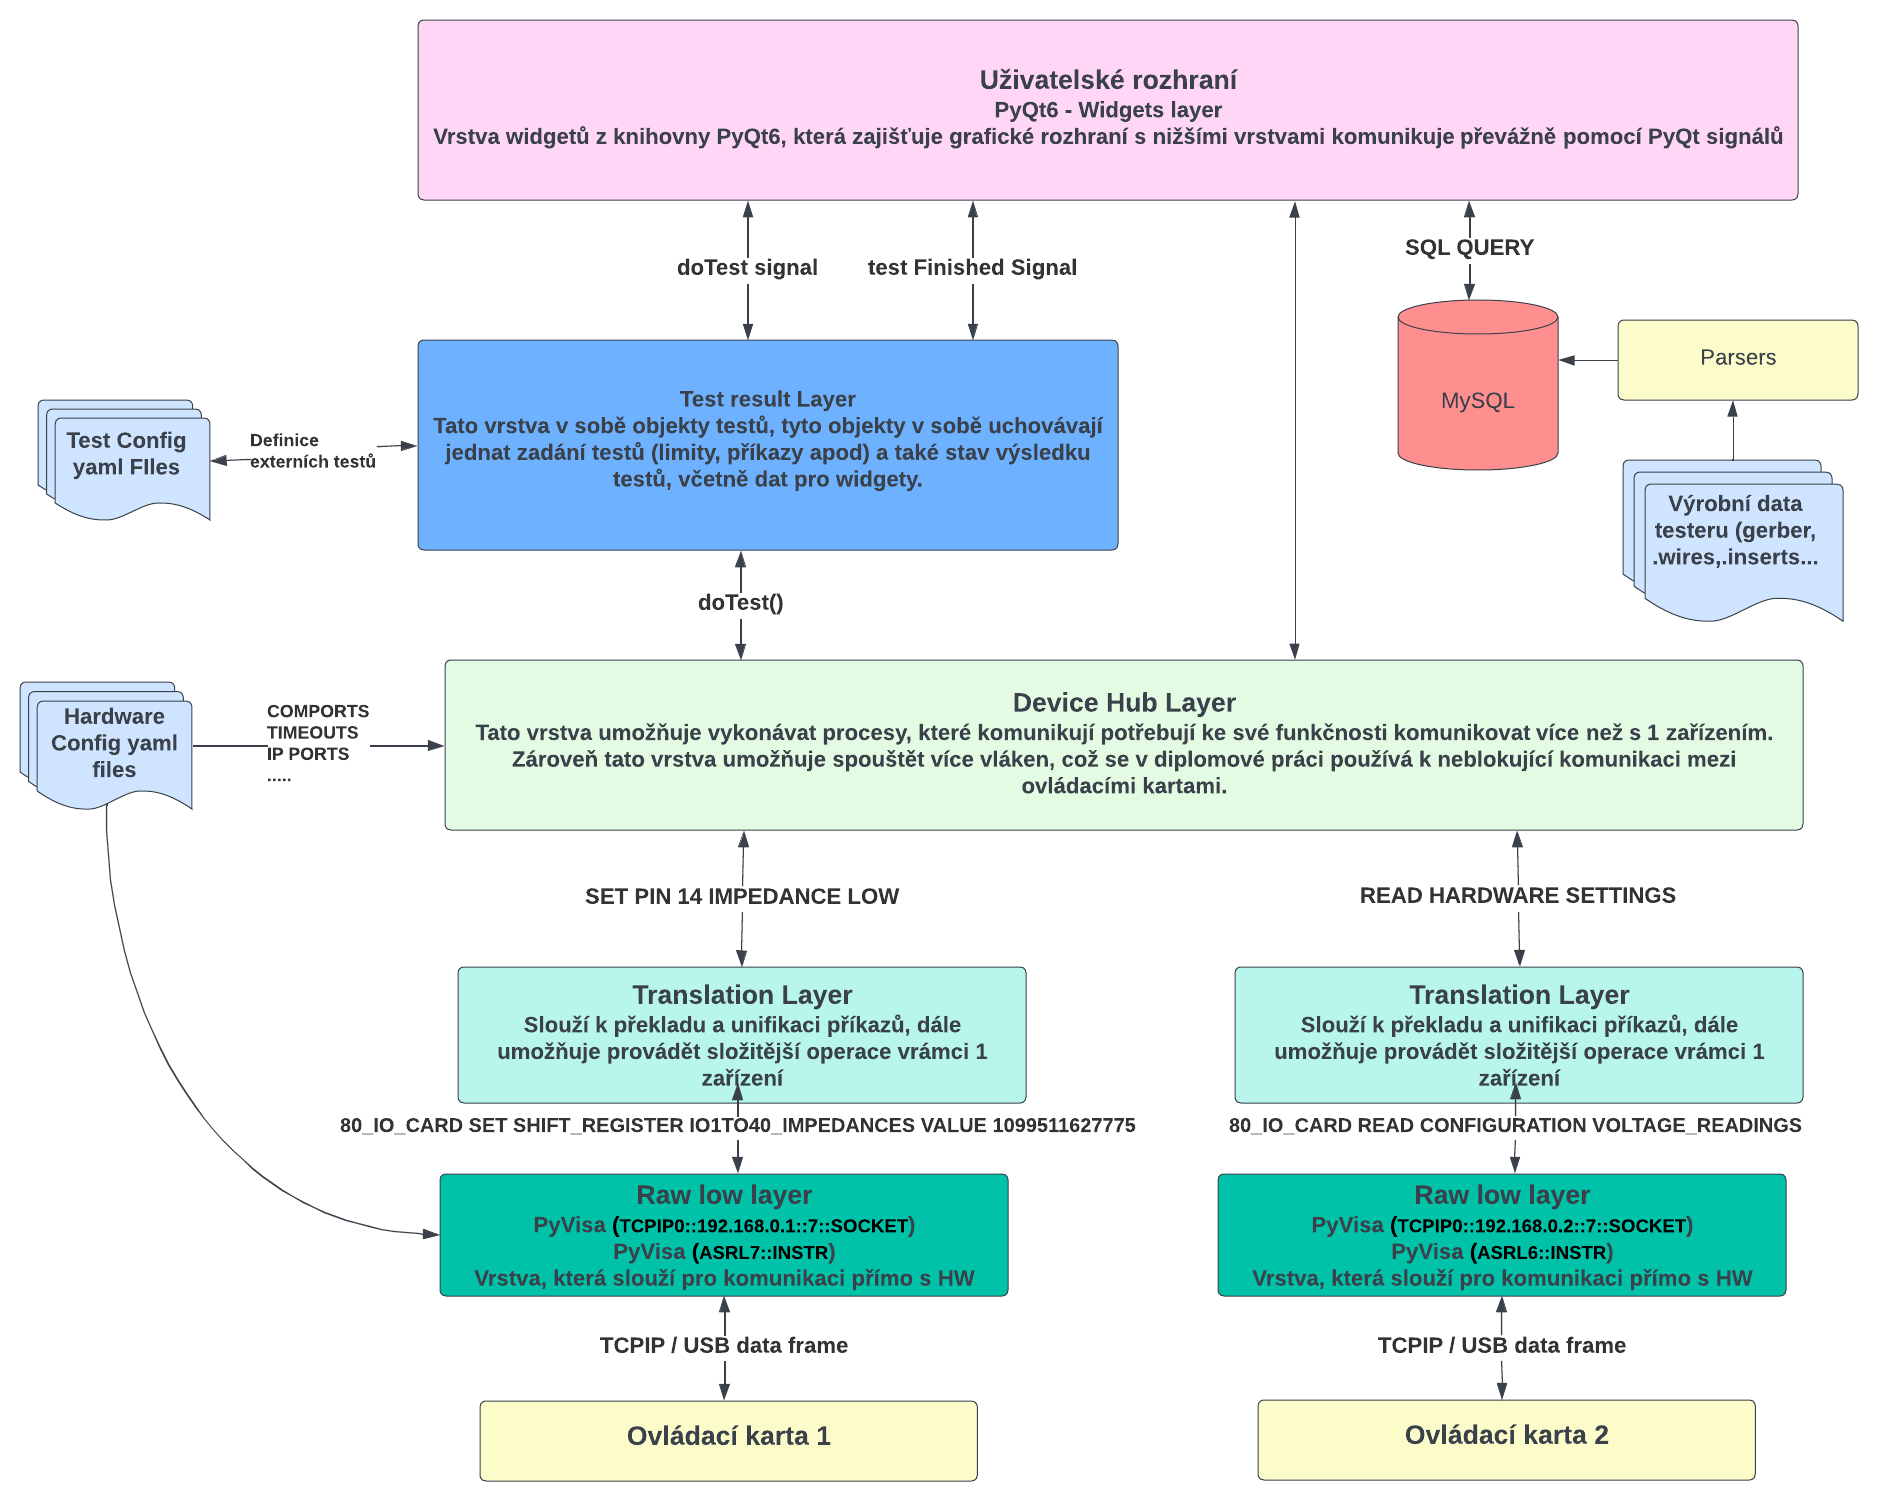
\includegraphics[width = 0.9\textwidth]{obrazky/PC_app_diagram.png}
    \caption{PC aplikace - top level diagram}
    \label{fig: PCAPP top level diagram}
\end{figure}


\section{PC aplikace - Raw low layer}
Nejnižší vrstvou je tzv. Raw low layer. Tato vrstva složí přímo ke komunikaci se zařízením. Převádí tak příkazy z kapitoly 4 do TCP/IP, popř. USB rámců.
V případě diplomové práce tuto vrstvu pro ovládací karty zajišťuje knihovna pyVisa, která je založena na knihovně VISA od firmy National Instruments.
Tato knihovna umožňuje pohodlně komunikovat se zařízením přes různé fyzické vrstvy (TCP/IP, USB, RS232, GPIB) a to pomocí jednotné API.\par


\section{PC aplikace - Translation Layer}
Druhou nejnižší vrstvou je tzv. Translation Layer (Překládací vrstva). Úkolem této vrstvy by mělo být poskytnout sofistikovanější funkce, které se skládají z více příkazů,
kterou nabízí komunikační protokol ovládaného zařízení. Zároveň by tato vrstva měla co nejvíce sjednocovat příkazy pro přístroje stejného druhu od různých výrobců.
Tato funkce je však pro diplomovou práci zanedbatelná, protože všechny ovládací karty používají stejný komunikační protokol.\par

Jako příklad funkce této vrstvy uveďme příkaz pro nastavení výstupní impedance pinu č.14 do nízké impedance, přičemž ostatní piny mají zůstat nezměněny.
Vyšší vrstvy předají příkaz v podobě SET PIN 14 IMPEDANCE LOW. Překládací vrstva nejprve zjistí aktuální hodnotu registru, který určuje impedance jednotlivých pinů.
Dále v závislosti na endianitě pozmění hodnotu registru a odešle příkaz, který nastaví novou hodnotu registru pomocí příkazu
80\_IO\_CAR SET SHIFT\_REGISTER IO1TO40\_IMPEDANCES VALUE "nová hodnota".\par


\section{PC aplikace - Device Hub Layer}
Device Hub Layer má za úkol vykonávat příkazy, které ke své funkci potřebují více než pouze jedno zařízení.
Typickým případem by bylo nastavení výstupního napětí napájecího zdroje a následné ověření napětí multimetrem.
V diplomové práci byla tato vrstva např. využita k automatizovanému měření průběhů v kapitole 4.\par

Druhým důležitým úkolem této vrstvy je rozřazovat požadované testy do vláken programu a předcházet tak zamrzání.
Z tohoto důvody by veškerá komunikace od vyšších vrstev měla probíhat přes tuto vrstvu.
Tato funkcionalita je vhodná pro diplomovou práci, protože umožňuje zasílat příkazy do několika ovládacích karet zároveň a
urychlit tak měření.


\section{PC aplikace - Test Result Layer}
Test Result layer je více než vrstvou spíše objektem.
Není tak striktně ohraničený a z historických důvodů má přesah do některých z nejnižších vrstev.
Do tohoto objektu jsou ukládány výsledky jednotlivých testů (příkazů) a zároveň jsou tyto výsledky vyhodnocovány podle
určitých kritérií.
Test Result Layer se nejčastěji uplatní v kombinaci s konfiguračním souborem tests.yaml, který není kompilován, má textovou podobu
a dokonce program lze kompilovat i v případě, že tento soubor neexistuje.
Následující obrázek je ukázkou výstřižku z konfiguračního souboru tests.yaml.

\subsection{konfigurační soubor tests.yaml}

\begin{figure}[ht!]
    \centering
    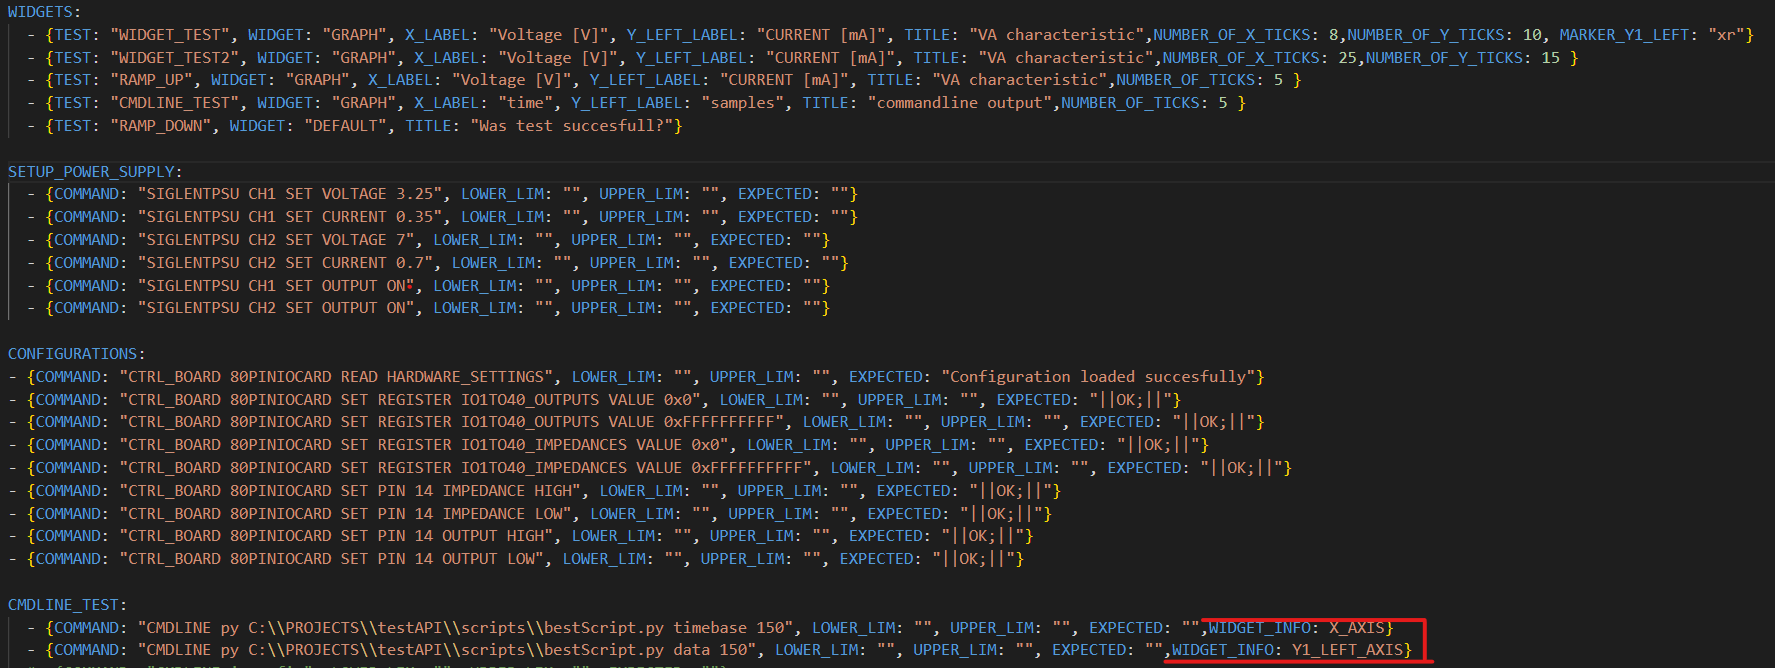
\includegraphics[width = 1\textwidth]{obrazky/test_result_class.png}
    \caption{PC aplikace - tests.yaml ukázka}
    \label{fig: tests yaml}
\end{figure}

Podrobný popis konfiguračního souboru test.yaml a všech jeho funkcí by byl příliš zdlouhavý.
Obecně jsou podporovány všechny příkazy, které nabízí Device Hub Vrstva.
Hlavní myšlenkou je demonstrovat, že pomocí tohoto souboru, lze dynamicky definovat testy a jejich widgety (způsob zobrazení). 
To, jaký widget bude použit pro zvolený test lze měnit v části "WIDGETS"\ tests.yaml souboru. Například pro test "CMDLINE\_TEST"\ je zvolen
widget "GRAPH", což v PC aplikaci nastaví zobrazení v podobě grafu.
Následně v červeně označené části (Obr. \ref{fig: tests yaml}) je definováno, která data budou zobrazena na určitých osách grafu.\par

Po spuštění testu lze v PC aplikaci zobrazit výsledky v následující podobě.
\begin{figure}[ht!]
    \centering
    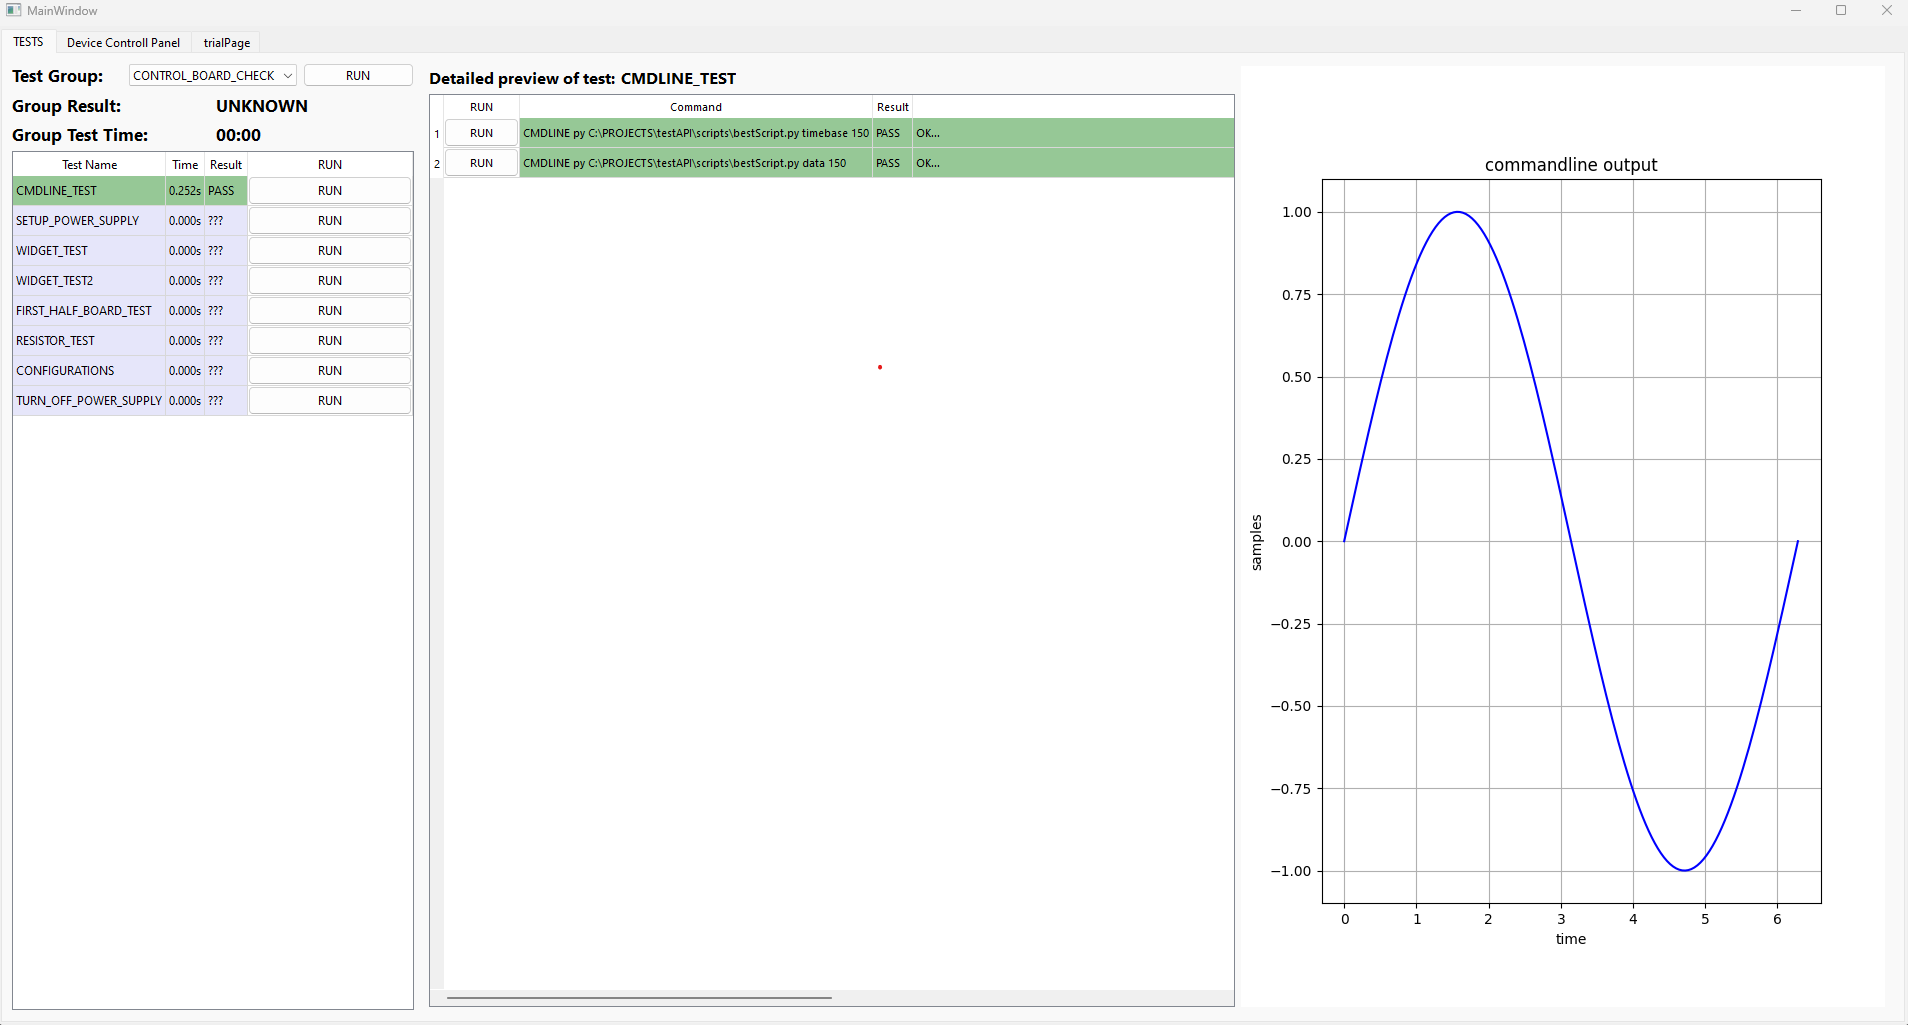
\includegraphics[width = 1\textwidth]{obrazky/test_result_widget_graph.png}
    \caption{PC aplikace - tests.yaml ukázka výsledku testů - graf}
    \label{fig: tests yaml graf}
\end{figure}

Pokud by byl spuštěn například test SETUP\_POWER\_SUPPLY, kterým mimo jiné byl nastavován laboratorní 
zdroj SIGLENT SPD3303X-E, pomocí kterého byla deska napájena v době měření všech výsledků zobrazených v diplomové práci.
PC aplikace zobrazí v pravé části výchozí widget, protože v konfiguračním souboru nebyl pro tento test žádný widget definován.
\begin{figure}[ht!]
    \centering
    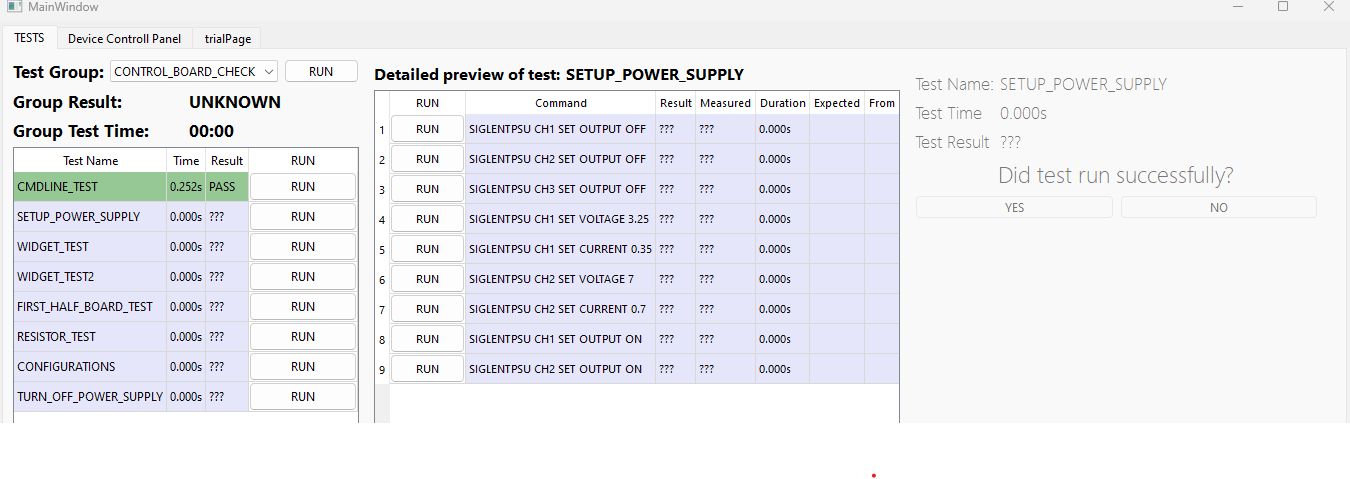
\includegraphics[width = 1\textwidth]{obrazky/test_result_widget_prompt.png}
    \caption{PC aplikace - tests.yaml ukázka výsledku testů - default}
    \label{fig: tests yaml default}
\end{figure}


\subsection{konfigurační soubor hardwareConfig.yaml}
Dalším konfiguračním souborem, který je v diplomové práci použit je soubor hardwareConfig.yaml. Tento soubor je oproti
předchozího souboru tests.yaml nutný k běhu programu. Nicméně jeho obsah je možné měnit i po kompilaci.
Následující obrázek je ukázkou výstřižku z tohoto souboru.
\begin{figure}[ht!]
    \centering
    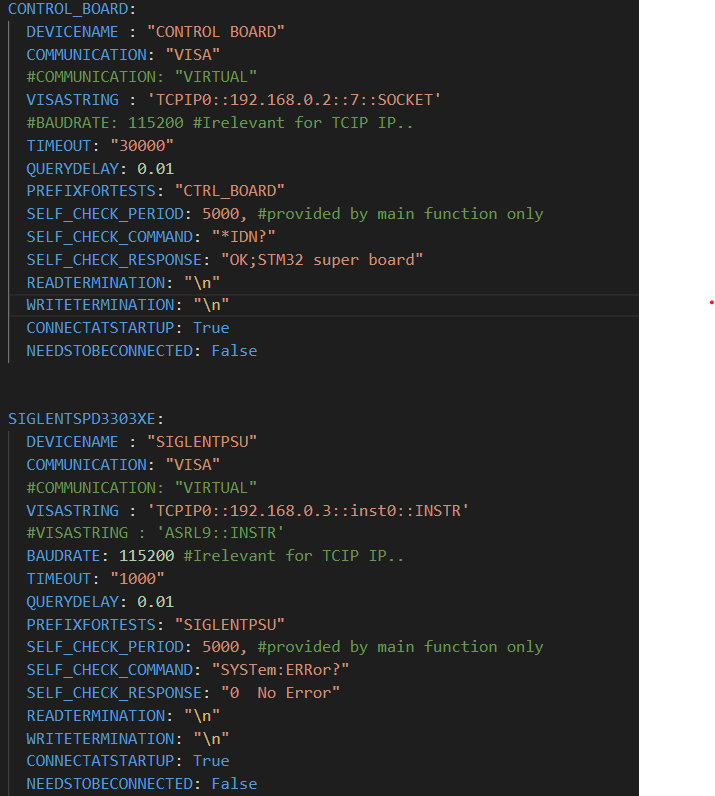
\includegraphics[width = 0.55\textwidth]{obrazky/hardwareConfig.png}
    \caption{PC aplikace - hardwareConfig.yaml}
    \label{fig: hardwareConfig yaml}
\end{figure}
\clearpage

Na výstřižku jsou zobrazeny konfigurace pro 2 zařízení, které používají pro Raw low layer právě komunikaci pomocí VISA knihoven.
Jsou zde nastaveny nejdůležitější parametry, které jsou potřebné pro komunikaci s daným zařízením. Zajímavou možností je zvolit
nastavení položky "COMMUNICATION"\ z VISA na VIRTUAL. Tímto lze aplikaci používat i v případě, že není k dispozici daný hardware.
Veškeré testy pro dané zařízení pak probíhají v tzv. "virtuálním módu". Pro některá zařízení je opravdu emulován virtuální hardware
a pro některá (včetně ovládacích karet z diplomové práce) jsou pouze navracovány hodnoty "VIRTUAL".\par

Důležitou položkou je parametr PREFIXFORTESTS, který určuje, jaký prefix bude použit pro testy, které jsou definovány v tests.yaml.
Například pro zmíněný test\linebreak
SETUP\_POWER\_SUPPLY z obrázku \ref{fig: tests yaml} je prefix "SIGLENTPSU". Každý test začínající na tento
prefix je pak přesměrován do příslušného hardwaru. V diplomové práci je využito těchto prefixů pro rozlišení jednotlivých ovládacích karet.

\section{PC aplikace - MySql databáze}
PC aplikace používá k ukládání data MySql databázi. Do databáze jsou ukládány jednak výsledky testů, tak databáze slouží jako sjednocovací
prvek pro výrobní data ICT testerů od různých výrobců. 
Výrobní data jsou převáděna pomocí různých parsovacích podprogramů do jednotné struktury databáze a zbylé části PC aplikace jsou pak nezávislé na
formátu výrobních dat. Tato struktura umožňuje jednoduše přidávat podporu pro další výrobce, pouze tvorbou nových parsovacích podprogramů.

\section{PC aplikace - Uživatelské rozhraní}
Uživatelské rozhraní PC aplikace je založeno na knihovně PyQt6. Tato knihovna je verzí knihovny Qt (originálně C++) pro jazyk Python.
PyQt6 umožňuje vytvářet různé widgety, které jsou mezi sebou propojovány pomocí signálů a slotů. Pro ovládací kartu bylo vytvořeno několik
widgetů. Všechny widgety diskutované v následujících sekcích jsou dostupné pro každou z připojených ovládacích karet.

\subsection{Widget - Visa terminal}
Prvním widgetem je VISA terminal, kde lze napřímo odesílat ovládací kartě příkazy z kapitoly č.4.

\begin{figure}[ht!]
    \centering
    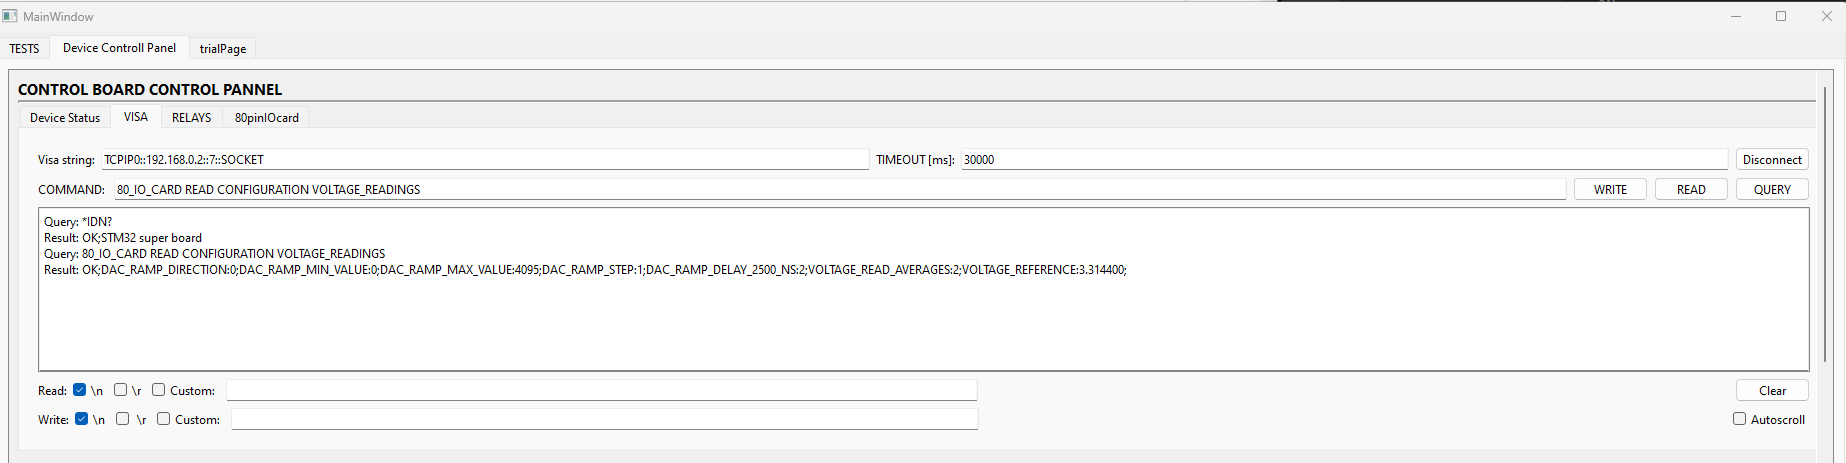
\includegraphics[width = 1\textwidth]{obrazky/PC_APP_VISA.png}
    \caption{PC aplikace - widget: VISA terminal}
    \label{fig: PCAPP VISA terminal}
\end{figure}

\subsection{Widget - Ovládání karty}
Další widget umožňuje pomocí grafického rozhraní nastavovat nejdůležitější funkce ovládacích karet. Na obrázku \ref{fig: PCAPP ovladani karty} lze vidět
ovládací panel, kde se pro každý pin dá nastavit jeho výstup či impedance.
Dále lze měřit napětí na jednotlivých pinech, získat aktuální logickou úroveň na pinu,
Nastavovat D/A převodník, vyčítat aktuální konfiguraci ovládací karty apod.

\begin{figure}[ht!]
    \centering
    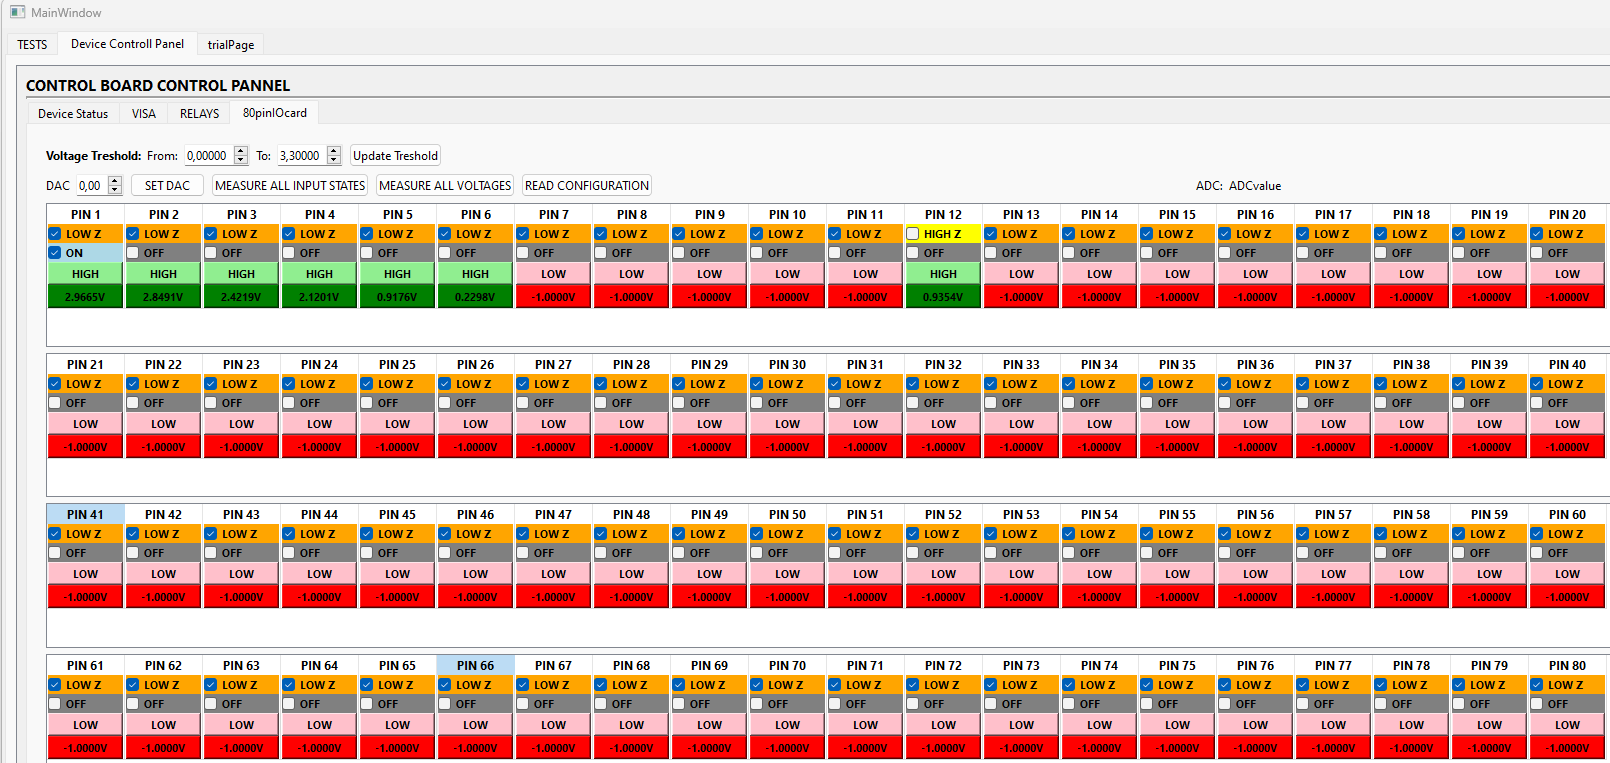
\includegraphics[width = 1\textwidth]{obrazky/PC_APP_CONTROL_PANEL.png}
    \caption{PC aplikace - widget: Ovládání karty}
    \label{fig: PCAPP ovladani karty}
\end{figure}

\subsection{Widget - Ovládání Relé}
Každá z ovládacích karet má k dispozici tzv. EXT porty, do kterých lze připojovat i jiné moduly než měřící karty diskutované v této diplomové práci.
Jedním z modulů, který je však využit je modul 32 relé karty připojený do EXT1 portu první ovládací karty. Tato relé karta slouží k ovládání mechanických
částí testeru jako jsou například vzduchové válce pro kontaktování apod. Na obrázku \ref{fig: PCAPP rele} lze vidět widget pro ovládání této relé karty.

\begin{figure}[ht!]
    \centering
    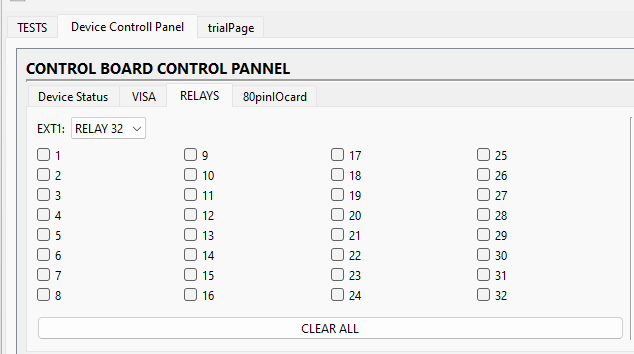
\includegraphics[height = 0.25\textheight]{obrazky/PC_APP_RELAY.png}
    \caption{PC aplikace - widget:  Relé}
    \label{fig: PCAPP rele}
\end{figure}


\subsection{Widget - Device status}
Každé z připojených zařízení má v aplikaci dostupný tzv. Device status widget, ve kterém jsou zobrazeny aktuální informace o
stavu daného zařízení. Také se v tomto widgetu vyskytuje tlačítko pro otevření příslušného konfiguračního souboru, pomocí kterého
lze modifikovat konfiguraci daného zařízení (Obr. \ref{fig: hardwareConfig yaml}). 

\begin{figure}[ht!]
    \centering
    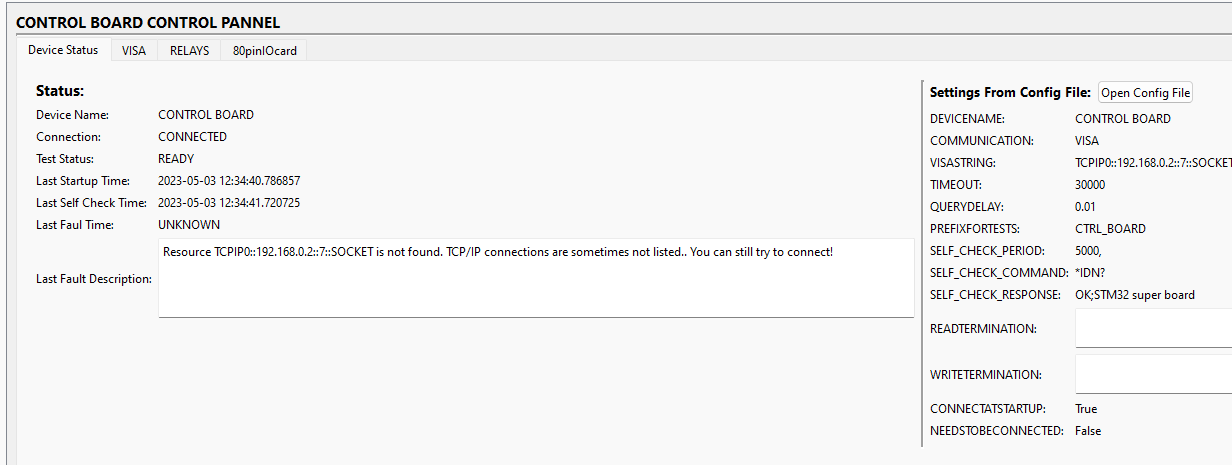
\includegraphics[width = 1\textwidth]{obrazky/Device_status.png}
    \caption{PC aplikace - widget:  Device status}
    \label{fig: PCAPP device status}
\end{figure}

\subsection{Widget - ICT propojení}
Widget ICT propojení je zobrazením dat uložených v MySQL databázi. V levé části tohoto widgetu (Pins And Probes), lze vidět všechny
bRC piny a testpointy. Po kliknutí na některý z těchto pinů se v prostřední části (Connections) zobrazí podrobné informace o vybraném pinu.
Pod detailními informacemi o pinu jsou zobrazena veškerá propojení,
která vedou z nebo do vybraného pinu. Pro každé propojení jsou zde i přídavné
informace o délce propojení, barvě drátu apod.\par
\begin{figure}[ht!]
    \centering
    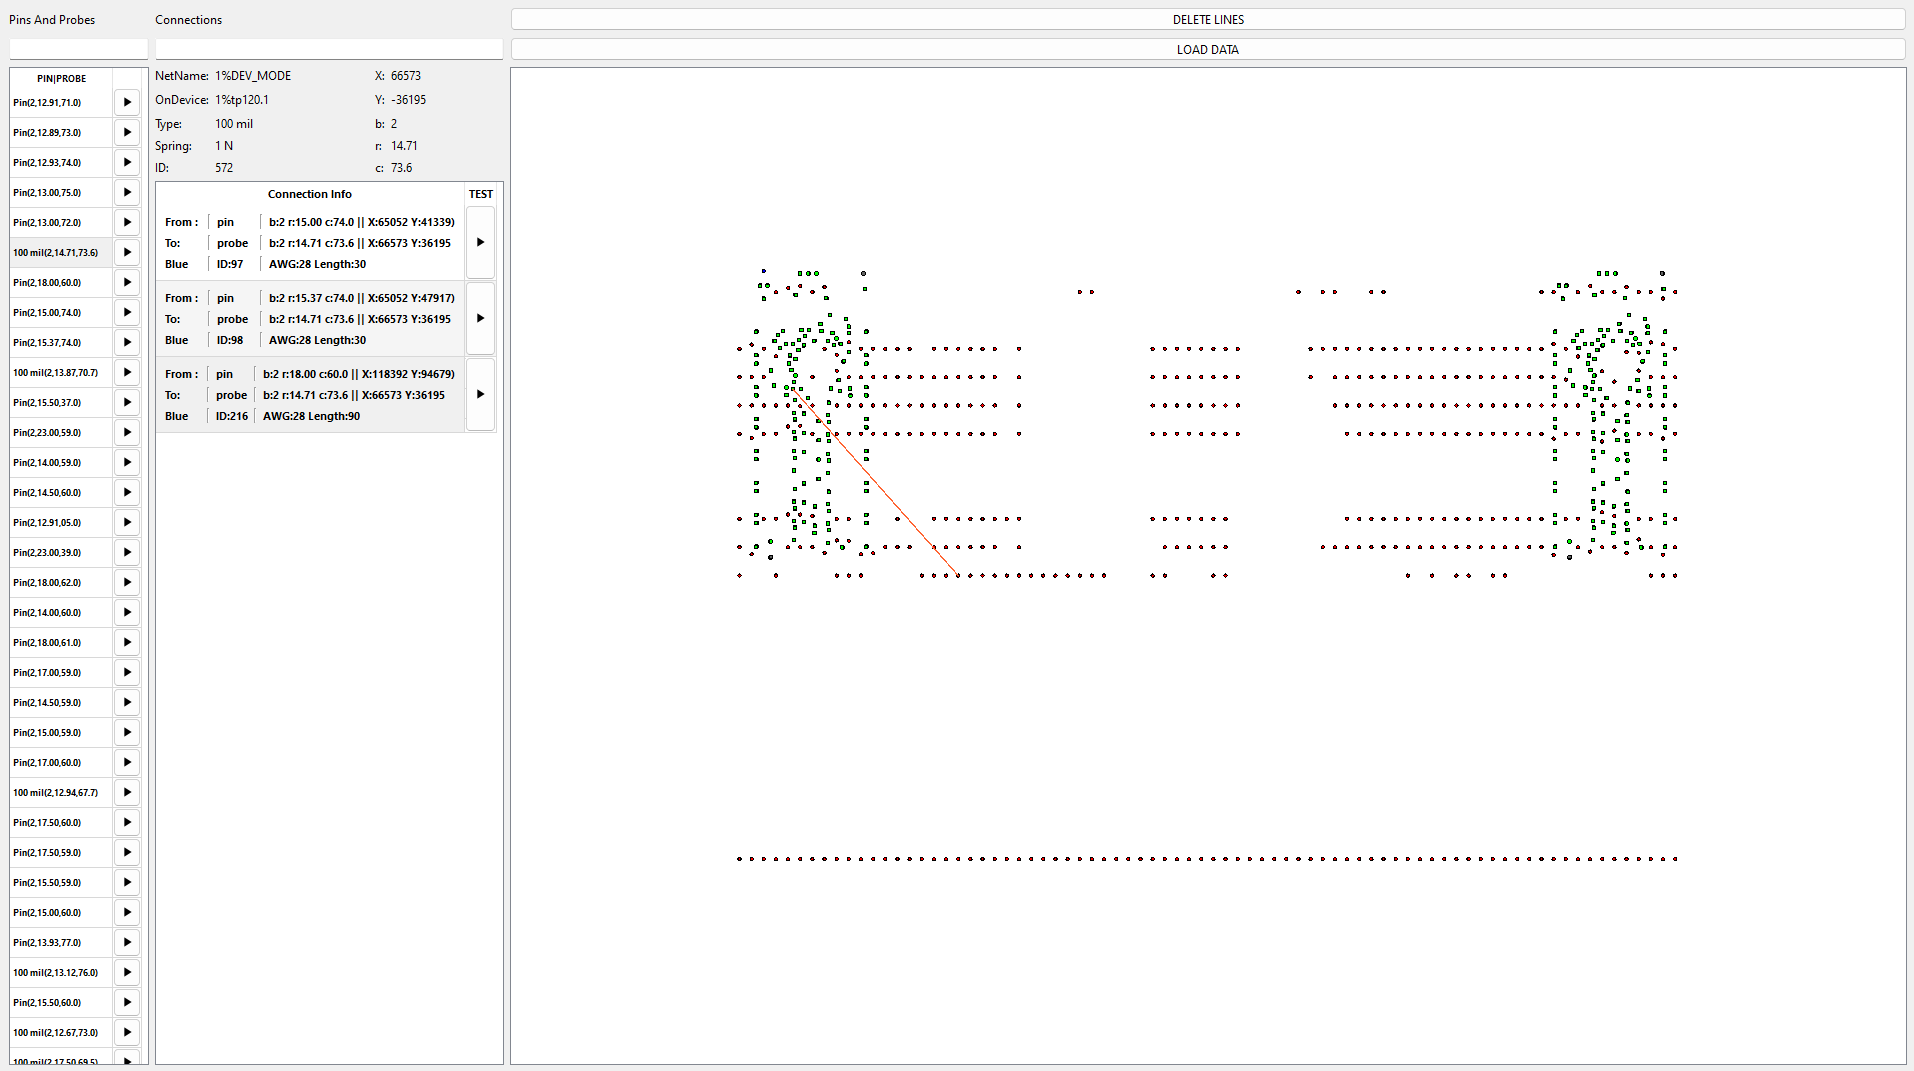
\includegraphics[height = 0.31\textheight]{obrazky/PC_APP_dataViewer.png}
    \caption{Widget:  ICT propojení}
    \label{fig: PCAPP ICT propojeni}
\end{figure}
\clearpage
Po kliknutí na některé z propojeních se v pravé části zobrazí grafické znázornění této cesty. Červenými kolečky jsou zde znázorněny jednotlivé bRC piny
na spodní straně fixture a zelenými čtverečky jednotlivé testpointy.\par

U každého z pinů (část Pins And Probes) i u každého z propojení (část Connections) je tlačítko s ikonou šipky. Po kliknutí na toto tlačítko
se provede příslušný test. Výsledky jsou pak interpretovány v podobě změny barev propojení. Červená barva značí, že propojení nevyhovuje nastaveným mezním hodnotám.
Zelená barva indikuje správné propojení. Oranžová barva je označením pro nesprávné propojení (vede na jiný pin než bylo zamýšleno).
V případě, že propojení zatím nebylo testováno, je propojení zobrazeno bezbarvě (bíle). Žlutá barva pak značí aktuálně vybrané propojení.

